\newpage
\section{Modalità allenamento}
La \textit{Modalità allenamento} permette a qualsiasi tipo di utente di allenarsi in uno degli argomenti proposti dal sistema. Dopo aver cliccato sul pulsante \textit{INIZIA L'ALLENAMENTO} presente nell'Home Page, viene presentata la seguente pagina:

\label{Modalità allenamento}
\begin{figure}[ht]
	\centering
	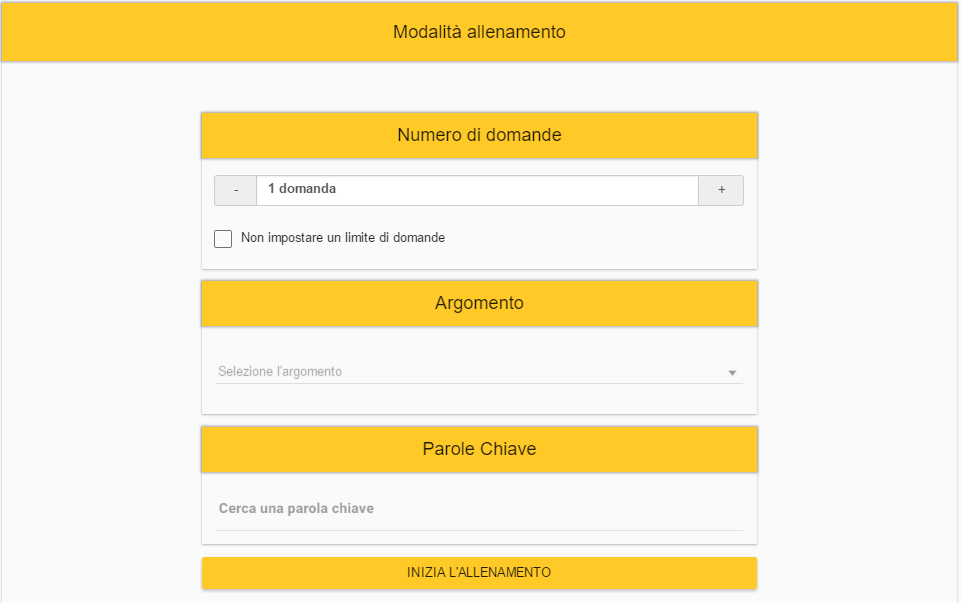
\includegraphics[scale=0.45]{img/allenamento.png}
	\caption{Modalità allenamento}
\end{figure}
\FloatBarrier

Prima di avviare un allenamento l'utente ha la possibilità di impostare i seguenti campi:
\begin{itemize}
	\item \textit{Numero di domande}: l'utente può impostare il numero massimo di domande che l'allenamento proporrà, oppure può decidere che non vi sia un limite prestabilito e avrà la possibilità di terminarlo quando vorrà;
	\item \textit{Argomento}: l'utente può selezionare l'argomento su cui verterà l'allenamento tra quelli proposti dal sistema;
	\item \textit{Parole chiave}: l'utente può ricercare le parole chiave a cui sono associate le domande e filtrarle così attraverso esse. Se ad esempio l'argomento selezionato è \textit{Patente} e la parola chiave ricercata è \textit{Guida}, il sistema proporrà domande relative all'argomento \textit{Patente} che hanno associata la parola chiave \textit{Guida}.
\end{itemize}

Terminata la compilazione dei campi sopra citati è possibile iniziare l'allenamento cliccando sul bottone \textit{INIZIA L'ALLENAMENTO}.